%% You can use this file to create your answer for Exercise 4  
%% Fill in the places labeled by comments.
%% Generate a PDF document by with the command `pdflatex ex4'.

\documentclass[11pt]{article}


\usepackage{times}
\usepackage{listings}
\usepackage{enumerate}
\usepackage{courier}
\usepackage{hyperref}
\usepackage{xcolor}
\usepackage{graphicx}
\usepackage{pdflscape}

%% Page layout
\oddsidemargin 0pt
\evensidemargin 0pt
\textheight 600pt
\textwidth 469pt
\setlength{\parindent}{0em}
\setlength{\parskip}{1ex}

%% Customization to listing
\lstset{basicstyle=\ttfamily\small,language=C,morekeywords={cilk_synch,cilk_spawn}}

%% Enumerate environment with alphabetic labels
\newenvironment{choice}{\begin{enumerate}[A.]}{\end{enumerate}}
\newenvironment{subchoice}{\begin{enumerate}[(1)]}{\end{enumerate}}
%% Environment for supplying answers to problem
\newenvironment{answer}{\begin{minipage}[c][2in]{\textwidth}}{\end{minipage}}

\begin{document}
\begin{flushright}                         
{\large\bf Full Name: \makebox[2in][l]{    
%% Put your name on the next line          
                                           
                                           
}} \\[1ex]                                 
                                           
{\large\bf Andrew Id: \makebox[2in][l]{\tt 
%% Put your Andrew ID on the next line     
                                           
}} \\[1ex]                                 
\end{flushright}                           
\vspace*{0.3in}                            
\begin{center}
\LARGE
15-418/618 \\
Exercise 4
\\ Answer Sheet % 
\end{center}

\section*{Problem 1: Lock Implementations}

\begin{choice}
\item Direct.

\begin{answer}
%% Provide your answer to 1A here
CAS direct always tries to write the lock and invalidates the cache in other processors. 
\end{answer}

\item Test.

\begin{answer}
%% Provide your answer to 1B here
CAS test only tries to write and invalidates after it detects the lock is 0. Before that, it 
only reads and don't invalidates. So it would be faster than CAS direct. 
\end{answer}


\item Backoff.

\begin{answer}
%% Provide your answer to 1C here

When a thread is in the delay, it won't even try to read. Thus it can be faster than CAS test. 

\end{answer}
\end{choice} 

\section*{Problem 2: Memory Consistency}

\begin{choice}
\item Explain why these two fence operations have such different
relative  performance.

\begin{answer}
%% Provide your answer to 2A here

As the number of threads grows, the contention over the global variable becomes more severe. 
However, the contends over the local variable still don't exist. So the differece between the 
two Implementations grows larger. 

\end{answer}

\item
Explain why the local version has performance that improves with the
number of threads.

\begin{answer}
%% Provide your answer to 2B here

The operation over local variable can all be paralleled. So with more threads, the time shared
by per operation is less. 
\textcolor{cyan}{The graph has an almost perfect speedup ($7.62\times$ for 8 threads). But the 
graph is not linear. The speedup is linear only means the proportion between two time is linear. }

\end{answer}

\item
For each of the five functions, determine where fence operations must be inserted
to guarantee the ordering properties.  You should insert only a
minimum set of fences.  Justify why these particular fences are
required and why no others are.

\begin{answer}
%% Provide your answer to 2C here
A fence should be used after the \lstinline{cas_lock_init} to ensure no write has happened 
before the write has done. 

A fence should be used before the \lstinline{cas_lock_unlock} to ensure all write operations
has finished before unlocking the lock. 

No need for fences in the lock functions. 
\end{answer}
\end{choice}

\section*{Problem 3: Interconnection Networks}

\begin{landscape}
\begin{figure}
\begin{center}
  %%  Provide your answer to Problem 3A by modifying the PDF file
  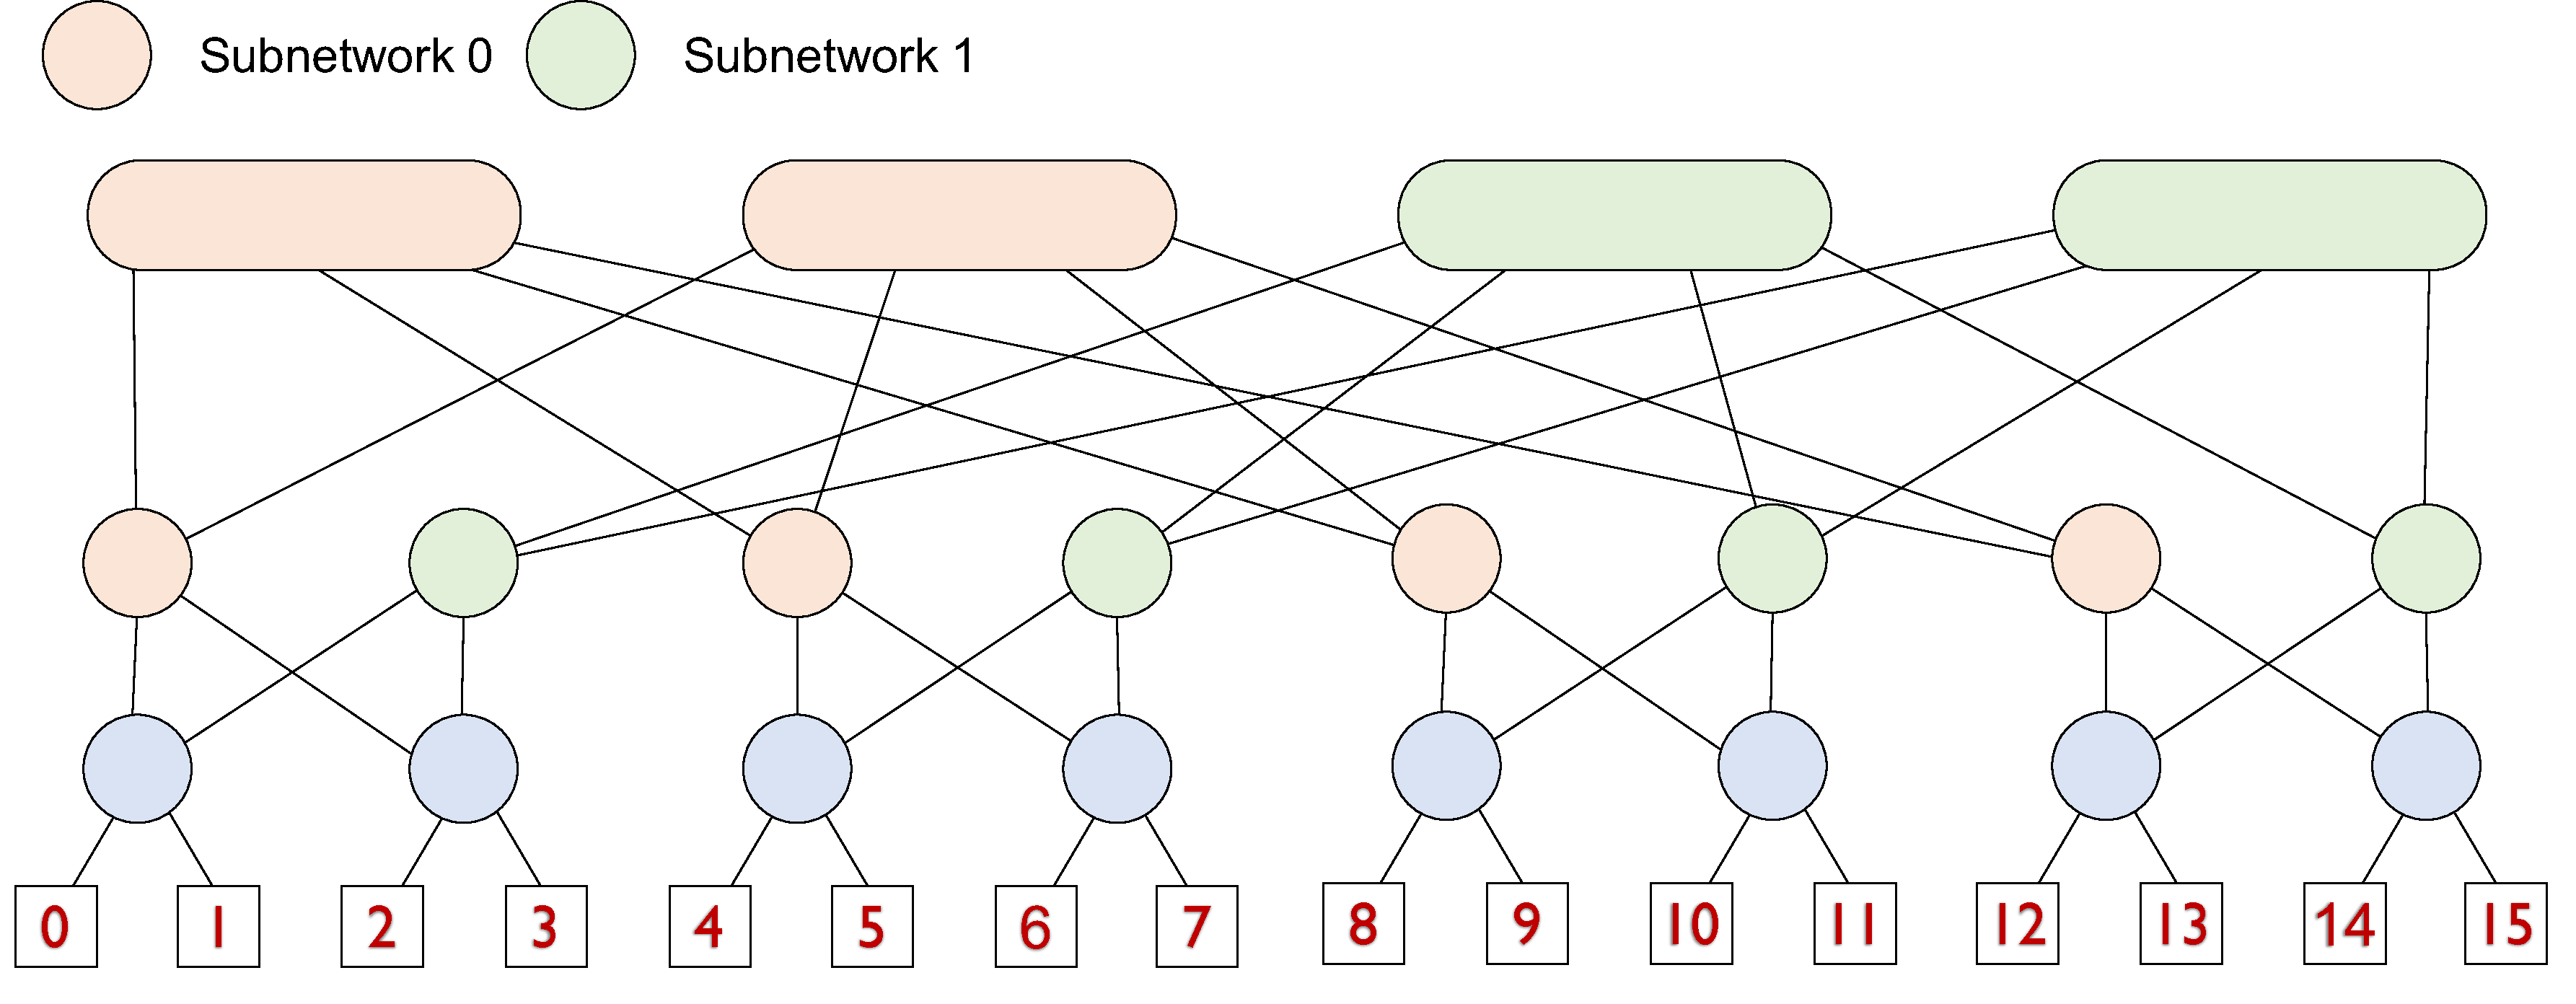
\includegraphics[width=9in]{figs/fat-tree.pdf} %% 
\end{center}
\caption{Fat-tree network, showing the recursive structure}
\label{fig:fat-tree}
\end{figure}
\end{landscape}

\begin{choice}
\item
Identify the $k/2$ subnetworks of type $N(k, 2)$ for $k = 4$ in Figure \ref{fig:fat-tree}.
You can do this by modifying the diagram
in Figure \ref{fig:fat-tree}.   Use different colors for the switches
to indicate the different subnetworks and the additional
switches.

\item
Derive a closed-form formula for $P(k, l)$.

\begin{answer}
%% Write your answer for Problem 3B here

$P(k,1)=k$

$P(k,l)=P(k,l-1) \cdot \frac{k}{2}$

Hence, $P(k, l)=P(k,1) \cdot (\frac{k}{2})^{(l-1)}=2(\frac{k}{2})^l$

\end{answer}

\item
Show that you could set up the eight links
forming a {\em mirror permutation}, mapping port $i$ to port $N-i-1$ for $0 \leq i < N/2$.
You can do this by modifying the diagram
in Figure \ref{fig:fat-tree-mirror}.  Use different colors to illustrate the different links.

\begin{landscape}
\begin{figure}
\begin{center}
%% Modify the provided figure to show the links using eight different colors
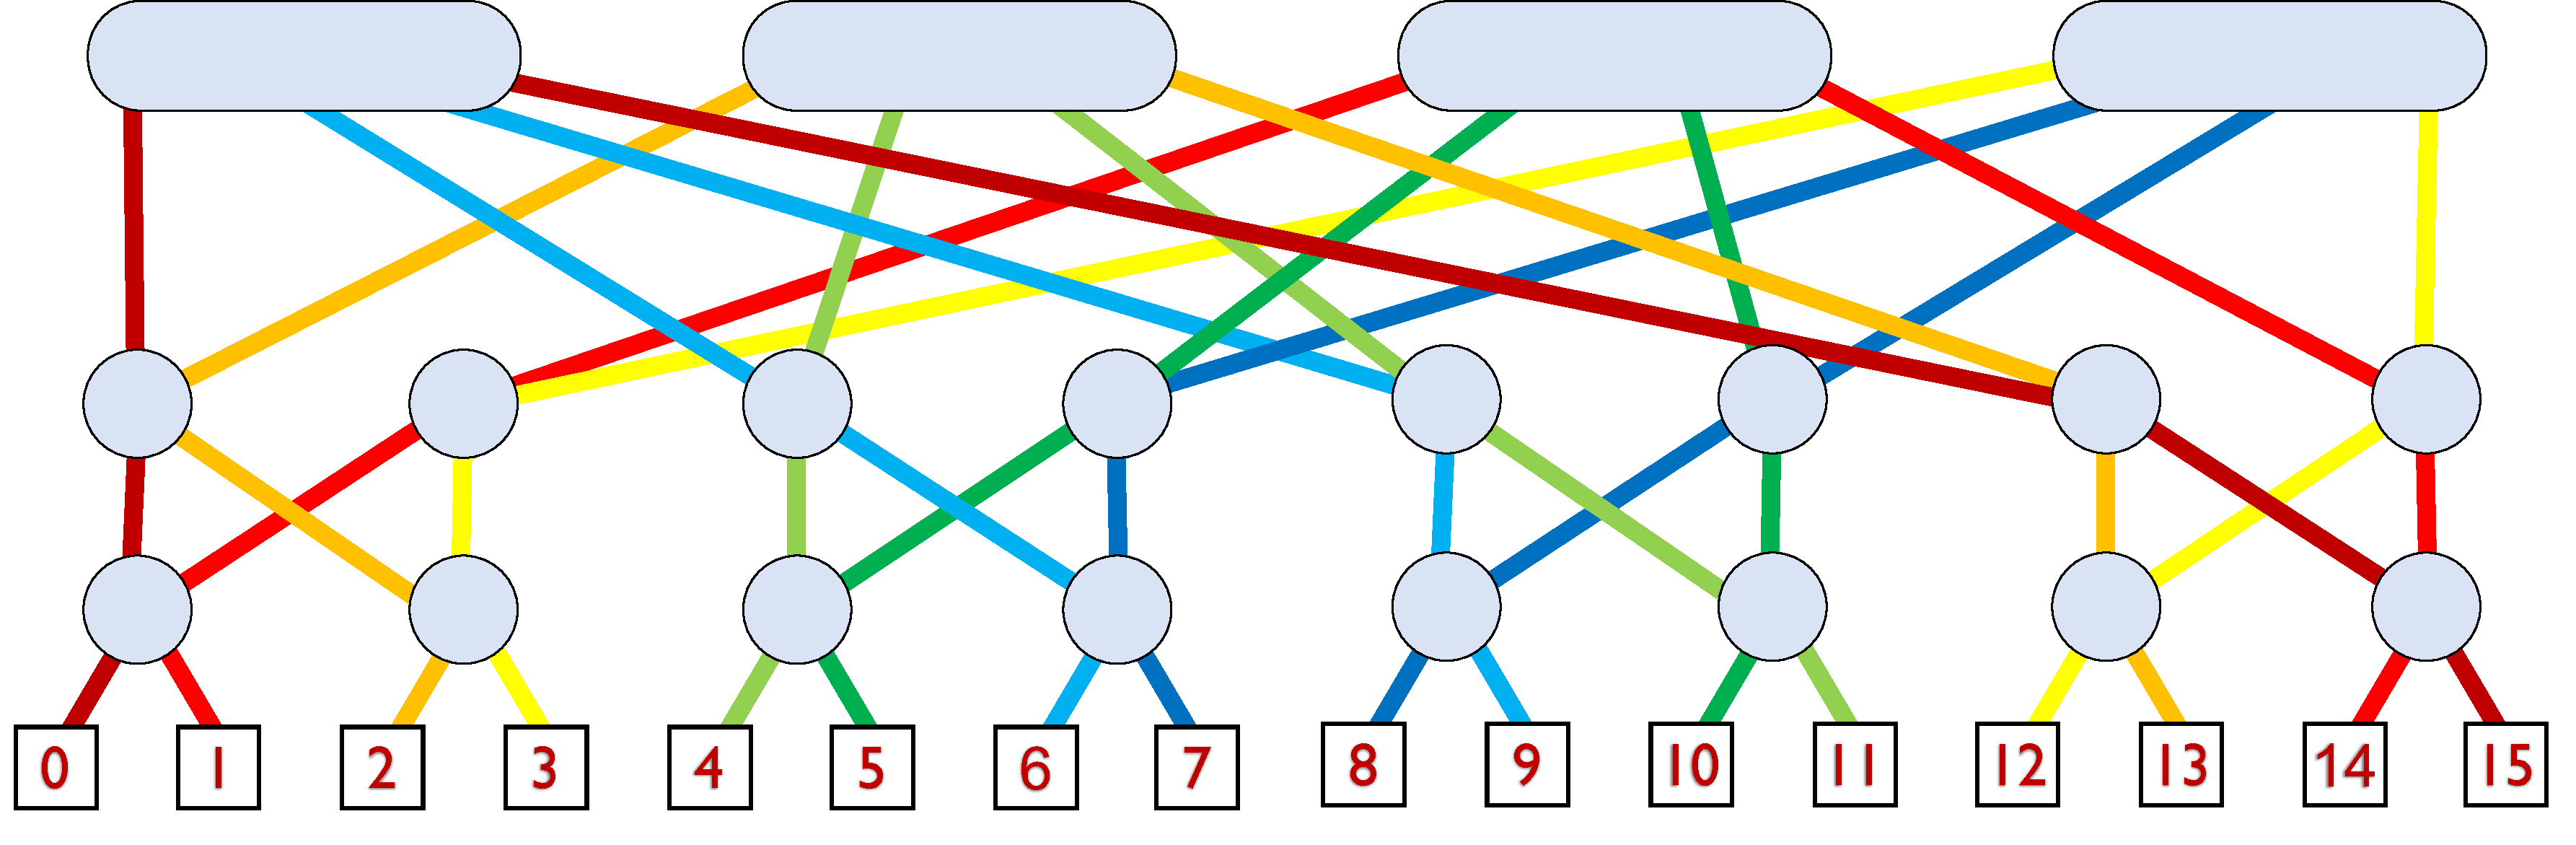
\includegraphics[width=9in]{figs/fat-tree-links.pdf} %% 
\end{center}
\caption{Fat-tree network with links for mirror permutation}
\label{fig:fat-tree-mirror}
\end{figure}
\end{landscape}
\end{choice}


\end{document}
